\subsubsection{Client}
La parte client della \DemoName{} è formata sostanzialmente dalle singole bubble, ognuna risiedente nel proprio package utente. Vi è inoltre la classe Client, che viene posta all'interno del componente Customer, data la correlazione con la bubble Customer.
\setclass{BubbleAndEat::Customer}
\paragraph[::Customer]{\class}\mbox{}\\ \label{\class}
\begin{figure}[H]
	\centering
	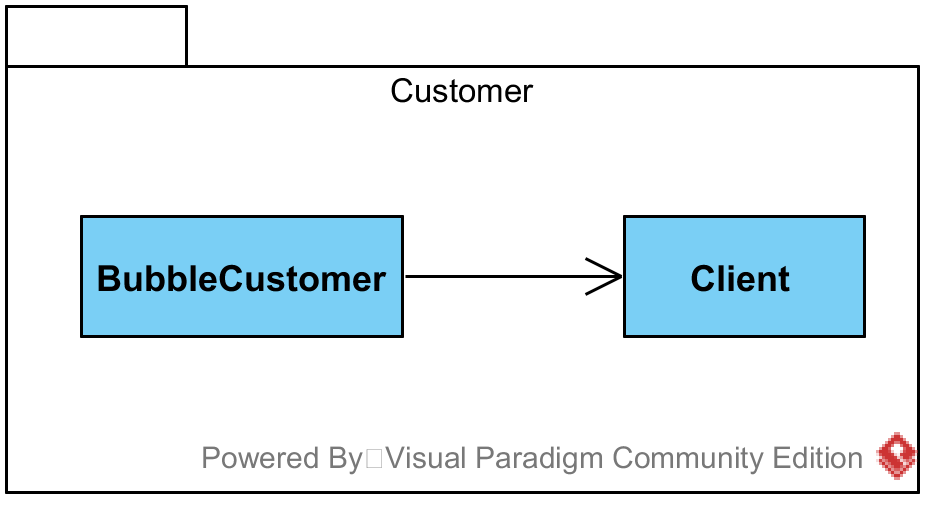
\includegraphics[width=7cm]{./diagrammi/demo/client/customer.png}
	\caption{Classe \class}
\end{figure}
Questo componente rappresenta il cliente e la sua bubble.

\setclass{BubbleAndEat::Customer::Client}
\subparagraph[::Client]{\class}\mbox{}\\ \label{\class}
\begin{figure}[H]
	\centering
	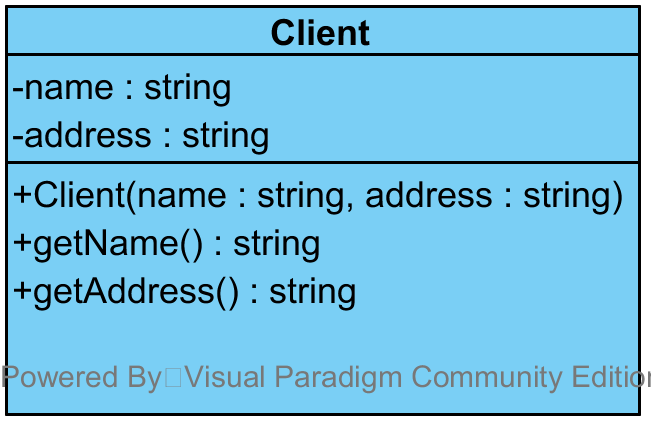
\includegraphics[width=7cm]{./diagrammi/demo/client/customer/client.png}
	\caption{Classe \class}
\end{figure}
\textbf{Descrizione:}\\
Classe che rappresenta un cliente.

\textbf{Utilizzo:}\\
Viene utilizzata per raccogliere le informazioni dei clienti.

%\textbf{Classi ereditate:}
%\begin{itemize}
%	\item \code{}.
%\end{itemize}
%
%\textbf{Sottoclassi:}
%\begin{itemize}
%	\item \coderef{}.
%\end{itemize}

\textbf{Attributi:}
\begin{itemize}
	\item \field{- name: string}: numero cliente;
	\item \field{- address: string}: indirizzo di spedizione.
\end{itemize}

\textbf{Metodi:}
\begin{itemize}
	\item \method{+ Client(name: string, address: string)}: costruttore, assegna i parametri;
	\begin{itemize}
		\item \param{name: string}: nome cliente;
		\item \param{address: string}: indirizzo di spedizione;
	\end{itemize}
	\item \method{+ getName(): string}: getter per \texttt{name};
	\item \method{+ setName(name: string): void}: setter per \texttt{name};
	\item \method{+ getAddress(): string}: getter per \texttt{address};
	\item \method{+ setAddress(address: string): void}: setter per \texttt{address}.
\end{itemize}

\setclass{BubbleAndEat::Customer::BubbleCustomer}
\paragraph[::BubbleCustomer]{\class}\mbox{}\\ \label{\class}
\begin{figure}[H]
	\centering
	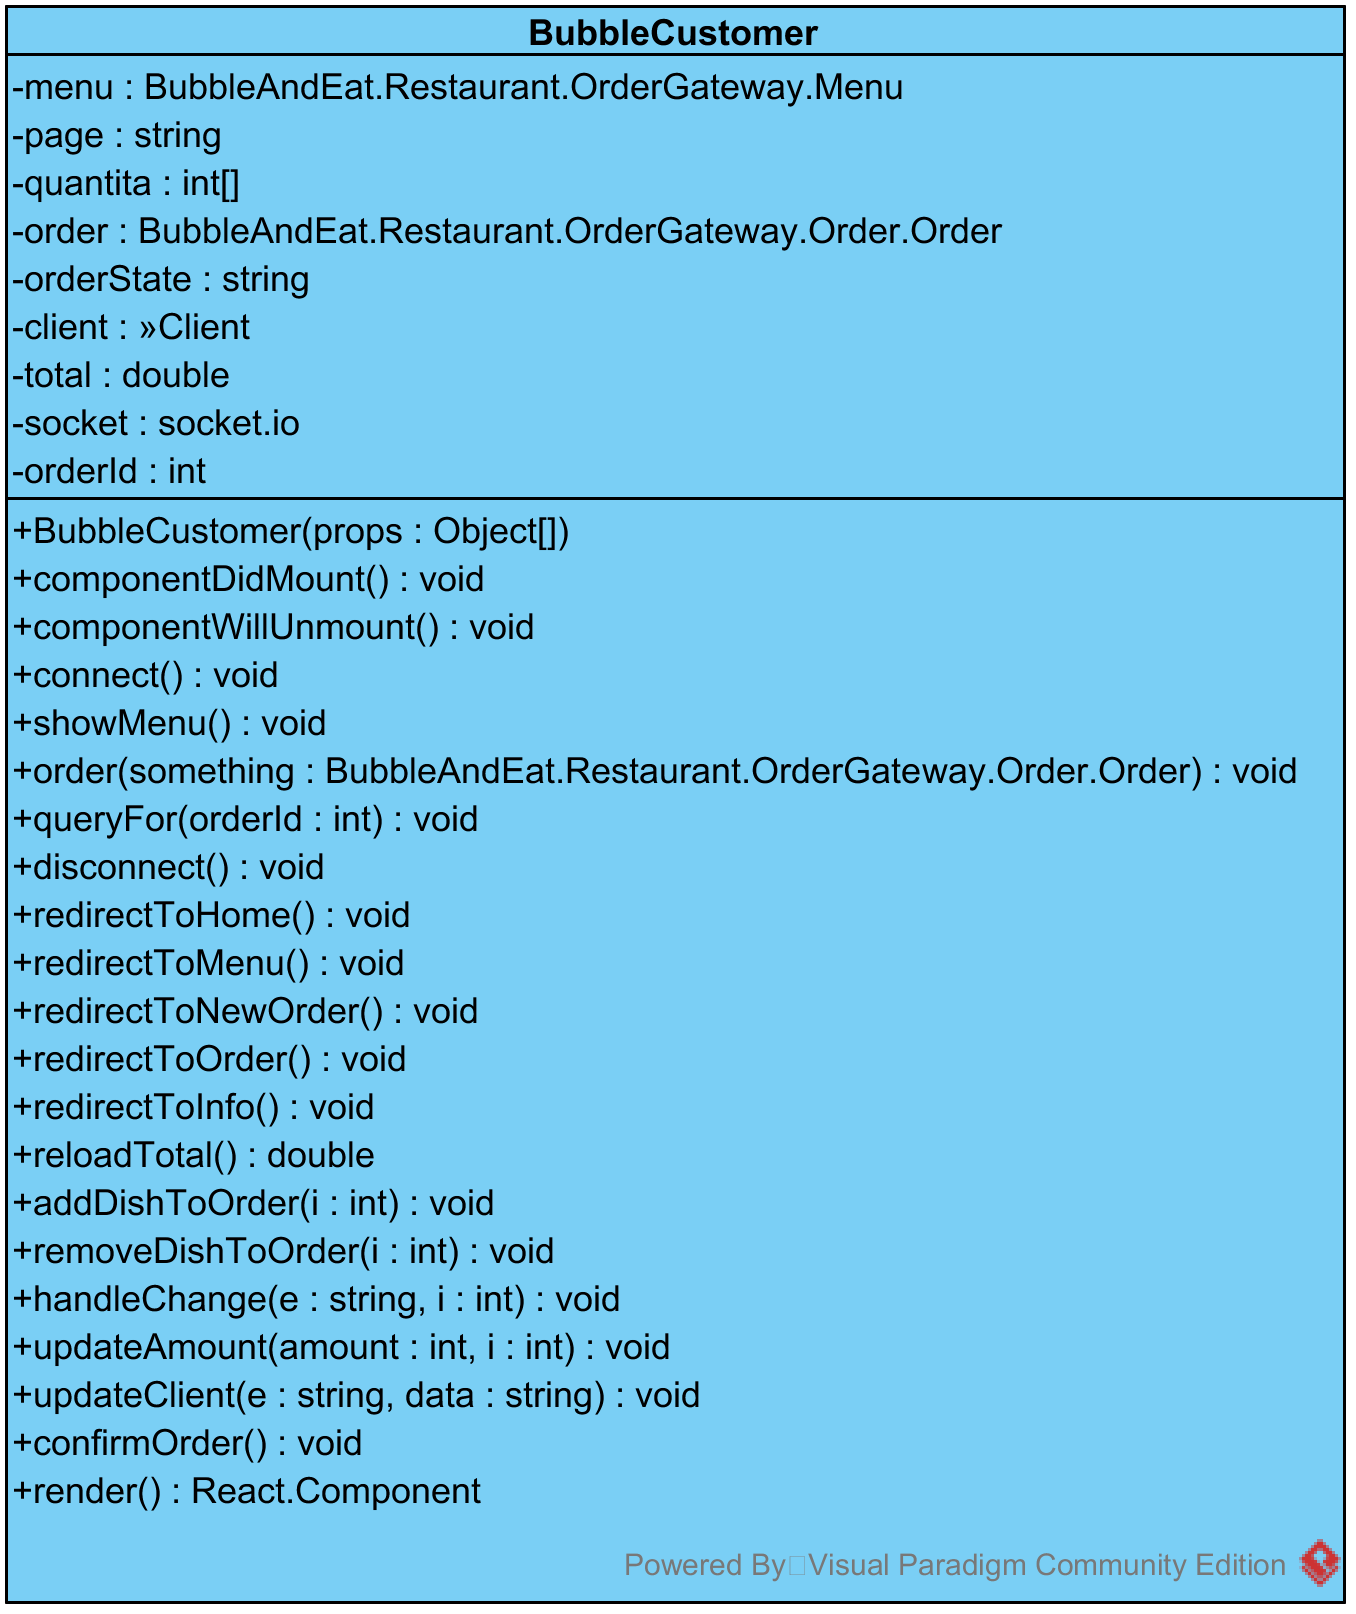
\includegraphics[width=12cm]{./diagrammi/demo/client/customer/bubblecustomer.png}
	\caption{Classe \class}
\end{figure}
\textbf{Descrizione:}\\
Classe che rappresenta il Customer e le sue funzionalità all'interno dell'applicazione.

\textbf{Utilizzo:}\\
Viene utilizzata per gestire le funzionalità dei clienti.

\textbf{Classi ereditate:}
\begin{itemize}
	\item \code{React::Component}.
\end{itemize}

%\textbf{Sottoclassi:}
%\begin{itemize}
%	\item \coderef{}.
%\end{itemize}

\textbf{Attributi:}
\begin{itemize}
%	\item \field{- props: Object[]}: array contenente le proprietà degli elementi della lista;
	\item \field{- menu: Menu}: menu del ristorante;
	\item \field{- page: string}: stringa che indica la pagina corrente;
	\item \field{- quantita: int[]}: array delle quantità dei diversi piatti presenti nell'ordinazione;
	\item \field{- order: Order}: oggetto che rappresenta l'ordine;
	\item \field{- orderState: string} stringa che indica lo stato dell'ordine;
	\item \field{- client: Client}: oggetto che rappresenta il cliente;
	\item \field{- total: double}: prezzo totale dell'ordine;
	\item \field{- socket: socket.io}: oggetto tramite il quale la classe gestisce la connessione con le altre componenti dell'applicazione;
	\item \field{- orderId: int}: id dell'ordine del cliente.
\end{itemize}

\textbf{Metodi:}
\begin{itemize}
	\item \method{+ CustomerBubble(props: Object[])}: costruttore, assegna i parametri;
		\begin{itemize}
			\item \param{props: Object[]}: array contenente le proprietà dei componenti React;
		\end{itemize}
	\item \method{+ componentDidMount(): void}: viene invocata alla creazione della classe e invoca la funzione connect;
	\item \method{+ componentWillUnmount(): void}: chiama il metodo disconnect alla distruzione della classe;
	\item \method{+ connect(): void}: connette la classe al resto dell'applicazione tramite socket;
	\item \method{+ showMenu(): void}: invia la richiesta di visualizzazione del menu;
	\item \method{+ order(something: Order): void}: invia l'ordine selezionato;
		\begin{itemize}
			\item \param{something: Order} l'ordine selezionato.
		\end{itemize}
	\item \method{+ queryFor(orderId: string): void}: invia la richiesta di informazioni sullo stato dell'ordine selezionato;
		\begin{itemize}
			\item \param{orderId: int}: id che identifica l'ordine.
		\end{itemize}
	\item \method{+ disconnect(): void}: libera le risorse quando viene distrutta la classe;
	\item \method{+ redirectToHome(): void}: renderizza e si sposta sulla pagina home;
	\item \method{+ redirectToMenu(): void}: renderizza e si sposta sulla pagina menu;
	\item \method{+ redirectToNewOrder(): void}: renderizza e si sposta sulla pagina di costruzione dell'ordine;
	\item \method{+ rediretToOrder(): void}: renderizza e si sposta sulla pagina di gestione dell'ordine; 
	\item \method{+ redirectToInfo() :void}: renderizza e si sposta sulla pagina info;
	\item \method{+ reloadTotal(): double}: ricalcola il prezzo totale e ne restituisce il valore;
	\item \method{+ addDishToOrder(i: int): void}: invoca updateAmount per aggiungere il piatto selezionato all'ordine;
		\begin{itemize}
			\item \param{i: int}: intero che identifica il piatto;
		\end{itemize}
	\item \method{+ removeDishToOrder(i: int): void}: invoca updateAmount per rimuovere il piatto selezionato dall'ordine;
		\begin{itemize}
			\item \param{i:int}: intero che identifica il piatto;
		\end{itemize}
	\item \method{+ handleChange(e: string, i: int): void}: gestisce un cambiamento manuale della quantità di un piatto;
		\begin{itemize}
			\item \param{e: Event}: evento;
			\item \param{i: int}: id del piatto.
		\end{itemize}
	\item \method{+ updateAmount(amount: int, i: int): void}: aggiorna le quantità dei diversi piatti;
	\item \method{+ updateClient(e: string, data: string): void}: aggiorna i dati del cliente;
		\begin{itemize}
			\item \param{e: Event}: evento avvenuto, contiene le nuove informazioni da inserire;
			\item \param{data: string}: indica il tipo di informazione modificata;
		\end{itemize}
	\item \method{+ confirmOrder(): void}: effettua l'ordine;
	\item \method{+ render(): React.Component}: renderizza la bubble.
\end{itemize}

\setclass{BubbleAndEat::Restaurant::Chef::BubbleChef}
\paragraph[::Restaurant::Chef::BubbleChef]{\class}\mbox{}\\ \label{\class}
\begin{figure}[H]
	\centering
	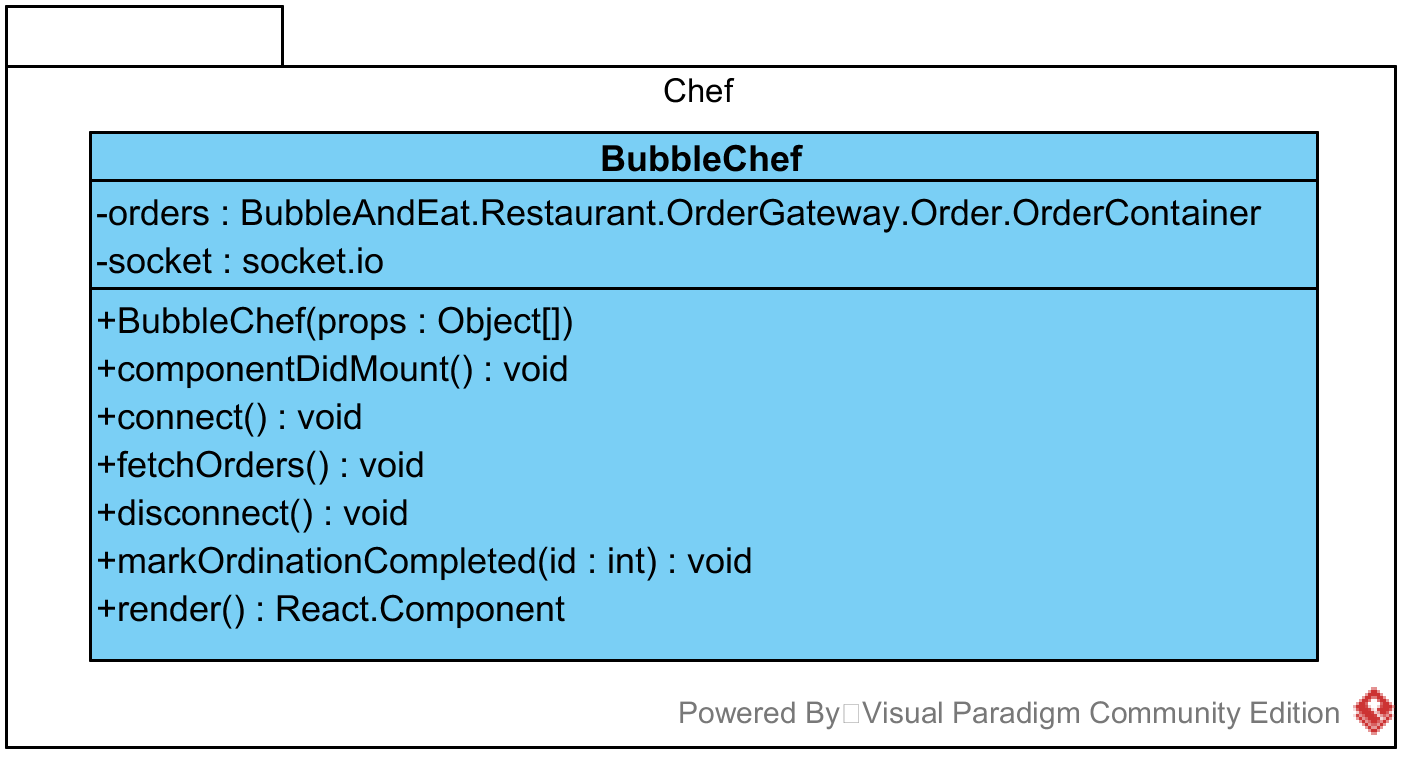
\includegraphics[width=12cm]{./diagrammi/demo/client/bubblechef.png}
	\caption{Classe \class}
\end{figure}
\textbf{Descrizione:}\\
Classe che rappresenta lo Chef e le sue funzionalità all'interno dell'applicazione.

\textbf{Utilizzo:}\\
Viene utilizzata per gestire le funzionalità dello Chef.

\textbf{Classi ereditate:}
\begin{itemize}
	\item \code{React::Component}.
\end{itemize}

%\textbf{Sottoclassi:}
%\begin{itemize}
%	\item \coderef{}.
%\end{itemize}

\textbf{Attributi:}
\begin{itemize}
	%	\item \field{- props: Object[]}: array contenente le proprietà degli elementi della lista;
	\item \field{- orders: OrderContainer}: contenitore delle ordinazioni da completare;
	\item \field{- socket: socket.io}: oggetto tramite il quale la classe gestisce la connessione con le altre componenti dell'applicazione.
\end{itemize}

\textbf{Metodi:}
\begin{itemize}
	\item \method{+ ChefBubble(props: Object[])}: costruttore, assegna i parametri;
	\begin{itemize}
		\item \param{props: Object[]}: array contenente le proprietà degli elementi;
	\end{itemize}
	\item \method{+ componentDidMount(): void}: viene invocata alla creazione della classe e invoca la funzione connect;
	\item \method{+ connect(): void}: crea la connessione con il server;
	\item \method{+ fetchOrders(): void}: invia la richiesta di visualizzazione delle ordinazioni;
	\item \method{+ disconnect(): void}: libera le risorse quando viene distrutta la classe;
	\item \method{+ markOrdinationCompleted(id: int): void}: indica come completata un'ordinazione;
		\begin{itemize}
			\item \param{id: int}: identifica l'ordine da completare;
		\end{itemize}
	\item \method{+ render(): React::Component}: renderizza la bubble.
\end{itemize}


\setclass{BubbleAndEat::Restaurant::Manager::BubbleManager}
\paragraph[::Restaurant::Manager::BubbleManager]{\class}\mbox{}\\ \label{\class}
\begin{figure}[H]
	\centering
	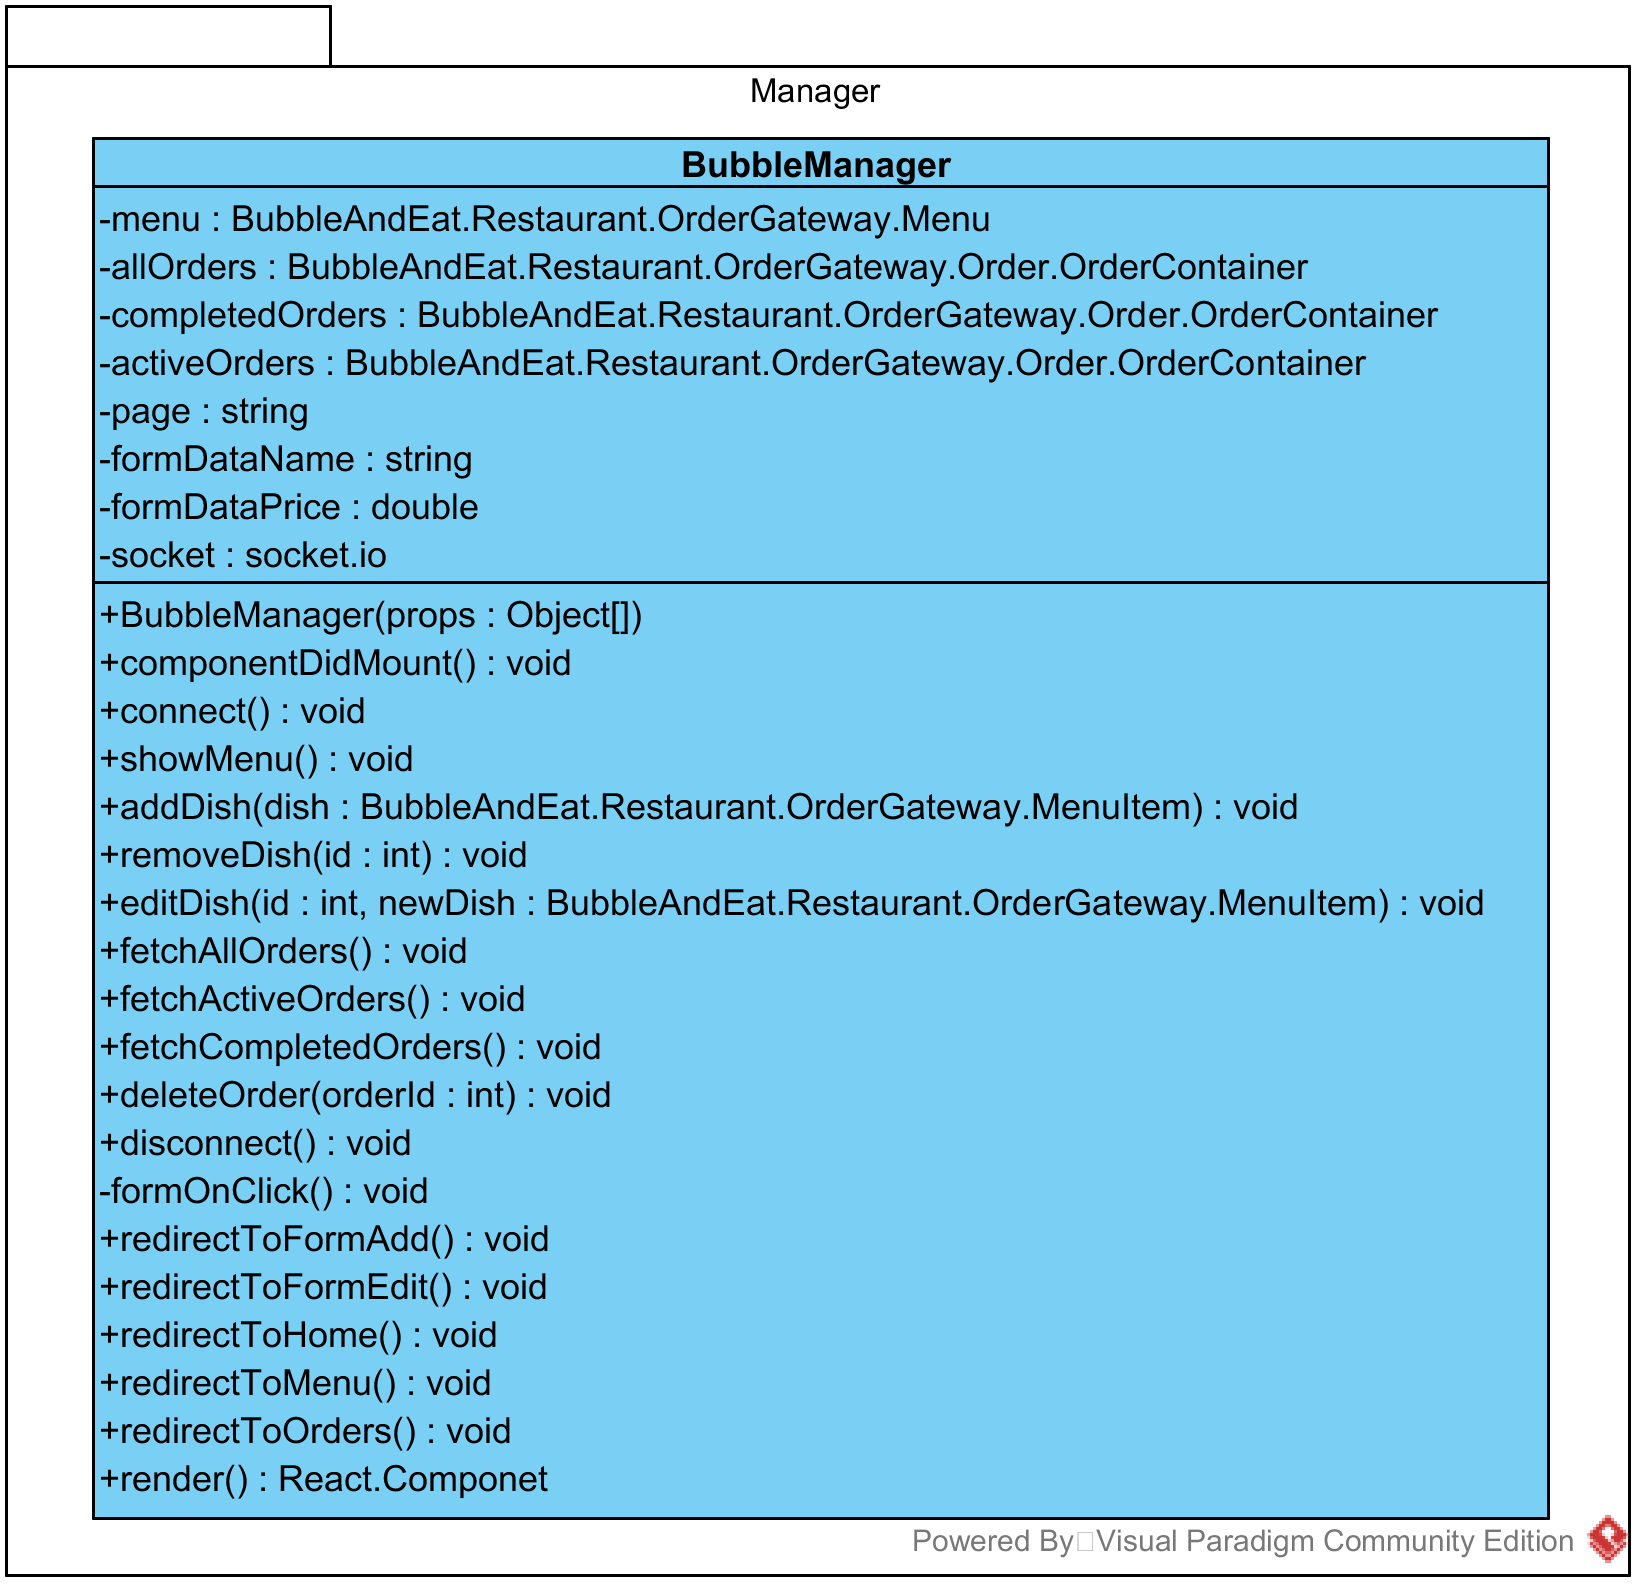
\includegraphics[width=14cm]{./diagrammi/demo/client/manager.png}
	\caption{Classe \class}
\end{figure}
\textbf{Descrizione:}\\
Classe che rappresenta la bubble del Manager.

\textbf{Utilizzo:}\\
Viene utilizzata per fornire all'utente Manager le funzionalità per egli disponibili.

\textbf{Classi ereditate:}
\begin{itemize}
	\item \code{React::Component}.
\end{itemize}
%
%\textbf{Sottoclassi:}
%\begin{itemize}
%	\item \coderef{}.
%\end{itemize}

\textbf{Attributi:}
\begin{itemize}
	\item \field{- menu: Menu}: menu del ristorante;
	\item \field{- allOrders: OrderContainer}: contenitore di tutti gli ordini esistenti nell'applicazione;
	\item \field{- completedOrders: OrderContainer}: contenitore di tutti e soli gli ordini completati;
	\item \field{- activeOrders: OrderContainer}: contenitore di tutti e soli gli ordini attivi (non completati);
	\item \field{- page: string}: pagina da renderizzare;
	\item \field{- formDataName: string}: valore contenuto nel campo \virgolette{Name} di creazione e modifica di una pietanza del menu;
	\item \field{- formDataPrice: double}: valore contenuto nel campo \virgolette{Price} di creazione e modifica di una pietanza del menu;
	\item \field{- socket: socket.io}: socket per la connessione al server.
\end{itemize}

\textbf{Metodi:}
\begin{itemize}
	\item \method{+ BubbleManager(props: Object[])}: costruttore, passa al costruttore della classe ereditata \texttt{props} e inizializza gli attributi con valori di default:
	\begin{itemize}
		\item \param{props: Object[]}: proprietà del componente React;
	\end{itemize}
	\item \method{+ componentDidMount(): void}: metodo invocato in automatico al caricamento della bubble, richiama in sè il metodo \texttt{connect};
	\item \method{+ connect(): void}: crea la connessione con il server;
	\item \method{+ showMenu(): void}: invia una richiesta al server per ricevere il menu aggiornato e lo assegna a \texttt{menu};
	\item \method{+ addDish(dish: MenuItem): void}: aggiunge una pietanza al menu e lo segnala al server;
	\item \method{+ removeDish(id: int): void}: rimuove una pietanza dal menu e lo segnala al server;
	\item \method{+ editDish(id: int, newDish: MenuItem): void}: modifica la pietanza con id \texttt{id} e lo segnala al server;
	\item \method{+ fetchAllOrders(): void}: invia una richiesta al server per ricevere il contenitore degli ordini aggiornato e lo assegna a \texttt{allOrders};
	\item \method{+ fetchActiveOrders(): void}: invia una richiesta al server per ricevere il contenitore degli ordini attivi e lo assegna a \texttt{activeOrders};
	\item \method{+ fetchCompletedOrders(): void}: invia una richiesta al server per ricevere il contenitore degli ordini completati e lo assegna a \texttt{completedOrders};
	\item \method{+ deleteOrder(orderId:int): void}: elimina un ordine e lo segnala al server:
	\begin{itemize}
		\item \param{orderId: int}: id dell'ordine da eliminare;
	\end{itemize}
	\item \method{+ disconnect(): void}: chiude la connessione con il server;
	\item \method{- formOnClick(): void}: definisce il comportamento della bubble quando viene azionato il \virgolette{submit} del form di aggiunta/modifica;
	\item \method{+ redirectToFormAdd(): void}: invoca la renderizzazione della pagina di aggiunta di una pietanza al menu;
	\item \method{+ redirectToFormEdit(): void}: invoca la renderizzazione della pagina di modifica di una pietanza al menu;
	\item \method{+ redirectToHome(): void}: invoca la renderizzazione della pagina principale della bubble;
	\item \method{+ redirectToMenu(): void}: invoca la renderizzazione della pagina di visualizzazione del menu;
	\item \method{+ redirectToOrders(): void}: invoca la renderizzazione della pagina di visualizzazione degli ordini;
	\item \method{+ render(): React::Component}: renderizza la bubble.
	
\end{itemize}